%%%%%%%%%%%%%%%%%%%%%%%%%%%%%%%%%%%%%%%%%
% Thin Sectioned Essay
% LaTeX Template
% Version 1.0 (3/8/13)
%
% This template has been downloaded from:
% http://www.LaTeXTemplates.com
%
% Original Author:
% Nicolas Diaz (nsdiaz@uc.cl) with extensive modifications by:
% Vel (vel@latextemplates.com)
%
% License:
% CC BY-NC-SA 3.0 (http://creativecommons.org/licenses/by-nc-sa/3.0/)
%
%%%%%%%%%%%%%%%%%%%%%%%%%%%%%%%%%%%%%%%%%

%----------------------------------------------------------------------------------------
%	PACKAGES AND OTHER DOCUMENT CONFIGURATIONS
%----------------------------------------------------------------------------------------

\documentclass[a4paper, 11pt]{article} % Font size (can be 10pt, 11pt or 12pt) and paper size (remove a4paper for US letter paper)

\usepackage[protrusion=true,expansion=true]{microtype}	% Better typography
\usepackage{graphicx} 		% Required for including pictures
\usepackage{wrapfig}  		% Allows in-line images
\usepackage{hyperref}		% Allows the use of hyperlinks
\usepackage{amsmath}
\usepackage{multirow}
\usepackage{rotating}
\usepackage{makecell}
\usepackage{diagbox}

\usepackage{mathpazo}		% Use the Palatino font
\usepackage[T1]{fontenc} 	% Required for accented characters
\usepackage[utf8]{inputenc}     % Spanish characters
\usepackage{amsmath} 		% Allows align
\usepackage{listings}		% Allows code 
\usepackage{float}		% Allows code 
\usepackage{subfig}


\lstset{basicstyle=\footnotesize\ttfamily,breaklines=true}

\linespread{1.05} % Change line spacing here, Palatino benefits from a slight increase by default

\makeatletter
\renewcommand\@biblabel[1]{\textbf{#1.}} % Change the square brackets for each bibliography item from '[1]' to '1.'
\renewcommand{\@listI}{\itemsep=0pt} % Reduce the space between items in the itemize and enumerate environments and the bibliography

\renewcommand{\maketitle}{ % Customize the title - do not edit title and author name here, see the TITLE block below
\begin{flushright} % Right align
{\LARGE\@title} % Increase the font size of the title

\vspace{50pt} % Some vertical space between the title and author name

{\large\@author} % Author name
\\\@date % Date

\vspace{40pt} % Some vertical space between the author block and abstract
\end{flushright}
}

%----------------------------------------------------------------------------------------
%	TITLE
%----------------------------------------------------------------------------------------

\title{\textbf{Clasificador Naive-Bayes}}

\author{
	\textsc{Agustín Mista}\\
	\textit{Universidad Nacional de Rosario}\\
 	\textit{Introducción a la Inteligencia Artificial}
}

\date{Rosario, 3 Junio de 2017}

%----------------------------------------------------------------------------------------

\begin{document}

\maketitle % Print the title section

%----------------------------------------------------------------------------------------
%	ABSTRACT
%----------------------------------------------------------------------------------------

%\renewcommand{\abstractname}{Summary} % Uncomment to change the name of the abstract to something else

%\begin{abstract}
%	Cuando todo esté cocinado, voy a completar este abstract con información pertinente.
%\end{abstract}

\vspace{20pt} % Some vertical space between the abstract and first section

%----------------------------------------------------------------------------------------
%	ESSAY BODY
%----------------------------------------------------------------------------------------

\section*{Introducción}

\begin{wrapfigure}{o}{0.45\textwidth}
	\begin{center}
		\vspace{-20pt}
		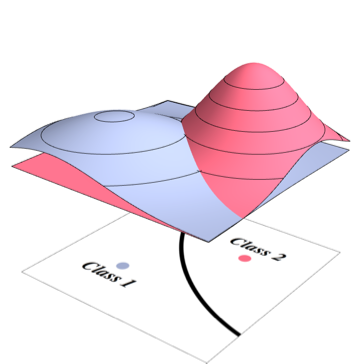
\includegraphics[width=0.4\textwidth]{bayes.png}
		\vspace{-20pt}
	\end{center}
\end{wrapfigure}

El objetivo de este trabajo práctico consta de analizar el funcionamiento de
los clasificadores probabilísticos basados en el Teorema de Bayes. Los mismos
son implementados teniendo en cuenta algunas hipótesis simplificadoras
adicionales sobre los datos a predecir. En un clasificador de Bayes
\text{ingenuo}, se asume que la presencia o ausencia de una característica no
está relacionada con la presencia o ausencia de cualquier otra, es decir, las
mismas se consideran independientes. Para el caso de nuestro análisis,
comparamos los resultados obtenidos con éste método en contraposición con otros
métodos de clasificación probabilistica antes vistos. Por otro lado, evaluamos
los resultados de éste clasificador para conjuntos de datos que ponen al límite
su capacidad. Los mismos luego son analizados nuevamente utilizando una versión
modificada del algoritmo que implementa un modelo de datos más adecuado.

\pagebreak

%------------------------------------------------

\section*{Apartado 2.}  \textbf{Dimensionalidad:}
\textit{Repita el punto 7 del Práctico 1, usando el Clasificador Bayesiano con
Gaussianas. Genere una gráfica incluyendo también los resultados de redes
neuronales artificiales y árboles de decisión.}\\

\vspace{20pt}

some blah more blah some blah more blah some blah more blah some blah more blah
some blah more blah some blah more blah some blah more blah some blah more blah
some blah more blah some blah more blah some blah more blah some blah more blah
some blah more blah some blah more blah some blah more blah some blah more blah
some blah more blah some blah more blah some blah more blah some blah more blah
some blah more blah some blah more blah some blah more blah some blah more blah
some blah more blah some blah more blah some blah more blah some blah more blah
some blah more blah some blah more blah some blah more blah some blah more blah
some blah more blah some blah more blah some blah more blah some blah more blah
some blah more blah some blah more blah some blah more blah some blah more blah 

\begin{figure}[H]
\captionsetup[subfigure]{justification=centering, labelformat=empty}
  \centering
  \subfloat[][]
           {\includegraphics[width=0.75\textwidth]{{bayes_vs_anns_vs_dtree}.png}}
\end{figure}

some blah more blah some blah more blah some blah more blah some blah more blah
some blah more blah some blah more blah some blah more blah some blah more blah
some blah more blah some blah more blah some blah more blah some blah more blah
some blah more blah some blah more blah some blah more blah some blah more blah
some blah more blah some blah more blah some blah more blah some blah more blah
some blah more blah some blah more blah some blah more blah some blah more blah
some blah more blah some blah more blah some blah more blah some blah more blah
some blah more blah some blah more blah some blah more blah some blah more blah
some blah more blah some blah more blah some blah more blah some blah more blah
some blah more blah some blah more blah some blah more blah some blah more blah 

%------------------------------------------------

\section*{Apartado 3.} \textbf{Límites del clasificador:}
\textit{Resuelva el problema de dos-elipses utilizando el Clasificador
Bayesiano con Gaussianas. Compare el resultado con el obtenido con redes.
Realice una gráfica de la predicción sobre el conjunto de test. Resuelva el
problema de las espirales-anidadas, y también compare con el resultado de redes
y realice la gráfica. Explique por qué se obtienen esos resultados.}\\

\vspace{20pt}

some blah more blah some blah more blah some blah more blah some blah more blah
some blah more blah some blah more blah some blah more blah some blah more blah
some blah more blah some blah more blah some blah more blah some blah more blah
some blah more blah some blah more blah some blah more blah some blah more blah
some blah more blah some blah more blah some blah more blah some blah more blah
some blah more blah some blah more blah some blah more blah some blah more blah
some blah more blah some blah more blah some blah more blah some blah more blah
some blah more blah some blah more blah some blah more blah some blah more blah
some blah more blah some blah more blah some blah more blah some blah more blah
some blah more blah some blah more blah some blah more blah some blah more blah 

\begin{figure}[H]
\captionsetup[subfigure]{justification=centering, labelformat=empty}
    \centering
    \caption*{\textbf{Prediccion usando Naive-Bayes:}}
    \subfloat[Dos elipses]
           {\includegraphics[width=0.5\textwidth]{{spiral.predic.bayes}.png}}
    \subfloat[Espirales anidadas]
           {\includegraphics[width=0.5\textwidth]{{dos_elipses.predic.bayes}.png}}
\end{figure}

\vspace{-20pt}
\begin{figure}[H]
\captionsetup[subfigure]{justification=centering, labelformat=empty}
    \centering
    \caption*{\textbf{Prediccion usando Redes Neuronales Artificiales:}}
    \subfloat[Dos elipses]
           {\includegraphics[width=0.5\textwidth]{{spiral.predic.ann}.png}}
    \subfloat[Espirales anidadas]
           {\includegraphics[width=0.5\textwidth]{{dos_elipses.predic.ann}.png}}
\end{figure}
\vspace{-20pt}
\begin{figure}[H]
\captionsetup[subfigure]{justification=centering, labelformat=empty}
    \centering
    \caption*{\textbf{Datos de prueba:}}
    \subfloat[Dos elipses]
           {\includegraphics[width=0.5\textwidth]{{spiral.test}.png}}
    \subfloat[Espirales anidadas]
           {\includegraphics[width=0.5\textwidth]{{dos_elipses.test}.png}}
\end{figure}

some blah more blah some blah more blah some blah more blah some blah more blah
some blah more blah some blah more blah some blah more blah some blah more blah
some blah more blah some blah more blah some blah more blah some blah more blah
some blah more blah some blah more blah some blah more blah some blah more blah
some blah more blah some blah more blah some blah more blah some blah more blah
some blah more blah some blah more blah some blah more blah some blah more blah
some blah more blah some blah more blah some blah more blah some blah more blah
some blah more blah some blah more blah some blah more blah some blah more blah
some blah more blah some blah more blah some blah more blah some blah more blah
some blah more blah some blah more blah some blah more blah some blah more blah 

%------------------------------------------------

\end{document}
